\section{Results}\label{results}

The tracking of the pupil works pretty well, as even in darker areas the pupil isn't lost. This can be seen in Fig.~\ref{fig:pupil1}.

\begin{figure}[h]
  \centering
  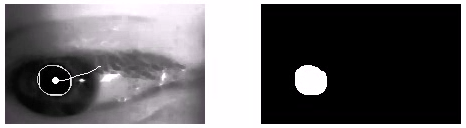
\includegraphics[width=0.9\textwidth]{fin_dark.png}
  \caption{Tracking of the pupil.}\label{fig:pupil1}
\end{figure}

When the eye movement is too strong, the pupil becomes the shape of an ellipse which is harder to find using \texttt{HoughCircles()} (Fig.~\ref{fig:pupillost}). In practice, movements this big do not occur.

\begin{figure}[h]
  \centering
  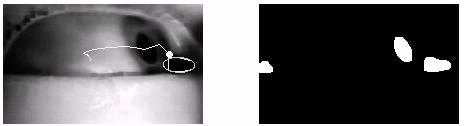
\includegraphics[width=0.9\textwidth]{fin_lost.png}
  \caption{The tracking is lost when the eyemovement is too strong.}\label{fig:pupillost}
\end{figure}

When the pupil isn't visible at all, the tracking looks for the darkest circle-like shape in the frame. Therefore the tracking also is off (Fig.~\ref{fig:pupilclosed}). As soon as the pupil is visible again, the algorithm finds it again.

\begin{figure}[h]
  \centering
  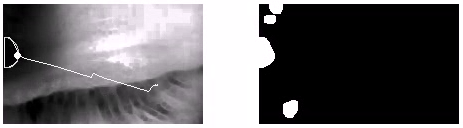
\includegraphics[width=0.9\textwidth]{fin_closed.png}
  \caption{The tracking is also lost when the eye is closed.}\label{fig:pupilclosed}
\end{figure}

The temporal filtering becomes apparent when the eye movement is very fast. This leads to a tracking, that lacks behing the actual pupil position (Fig.~\ref{fig:pupiltemporal}). This makes the tracking smoother but also a bit slower.

\begin{figure}[h]
  \centering
  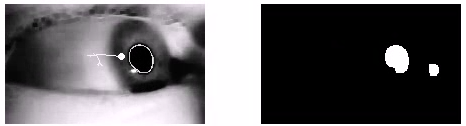
\includegraphics[width=0.9\textwidth]{fin_temporal.png}
  \caption{For fast movements the effect of the temporal filtering becomes apparent.}\label{fig:pupiltemporal}
\end{figure}

In the calibration routine as shown in Fig.~\ref{fig:calibration} the homography is estimated.

\begin{figure}[h]
  \centering
  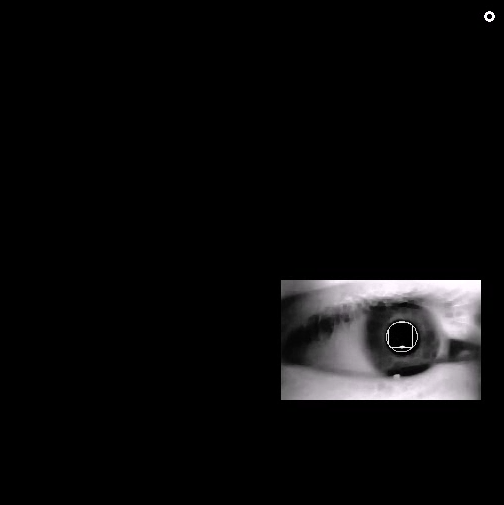
\includegraphics[width=0.5\textwidth]{fin_calibration.png}
  \caption{Calibration sequence.}\label{fig:calibration}
\end{figure}

After the homography is estimated, the mapping can be performed as illustrated in Fig~\ref{fig:mapping}.

\begin{figure}[h]
  \centering
  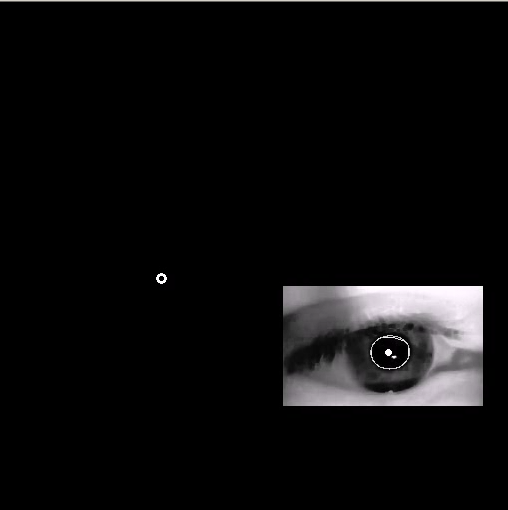
\includegraphics[width=0.5\textwidth]{fin_mapping.png}
  \caption{The mapping maps the eye position onto the screen.}\label{fig:mapping}
\end{figure}

Figure~\ref{fig:headmarkers} shows the tracking of the four markers mounted on the spectacle frame.

\begin{figure}[h]
  \centering
  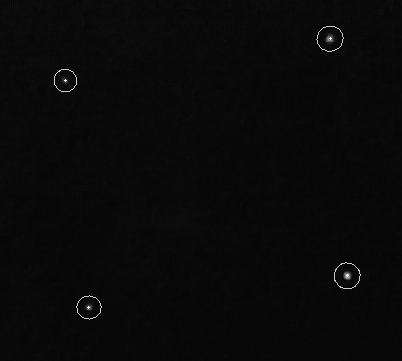
\includegraphics[width=0.9\textwidth]{fin_head.png}
  \caption{Tracking of the four markers.}\label{fig:headmarkers}
\end{figure}

To get an idea of the whole process, please see the attached video. This video first shows how the eye tracking works in general. Some problems are shown as well, for instance the behaviour of the pupil tracking when the eye is closed or when the eye movement is too big and the tracking can not distinguish between the pupil and shadows. Keep in mind that movements this big do not occur in normal usage, as the movement of the eye is rather limited when looking at a computer screen.

The next part shows the calibration process, where the user has to look at several points on the screen.

After his process, all the necessary information is gathered to perform the mapping, which is shown subsequently. The user looks at several points on the screen and the position of the pupil is mapped onto the screen. 

The result shown in this video lacks the head tracking, as we weren't able to implement this properly due to several tough problems. These problems are discussed in the next section.


